\section{Methodology}
\label{sec:method}

This section details the mathematical and architectural formulation of \textbf{FRAME}. Given a single unconstrained RGB image, FRAME estimates whether the image contains an AI-generated local edit and computes a dense, pixel-accurate localization mask. The system operates strictly without access to the original unedited photograph or reference masks at deployment. Figure~\ref{fig:framework_flowchart} illustrates the overall architecture and operational dataflow.

\begin{figure*}[t]
\centering
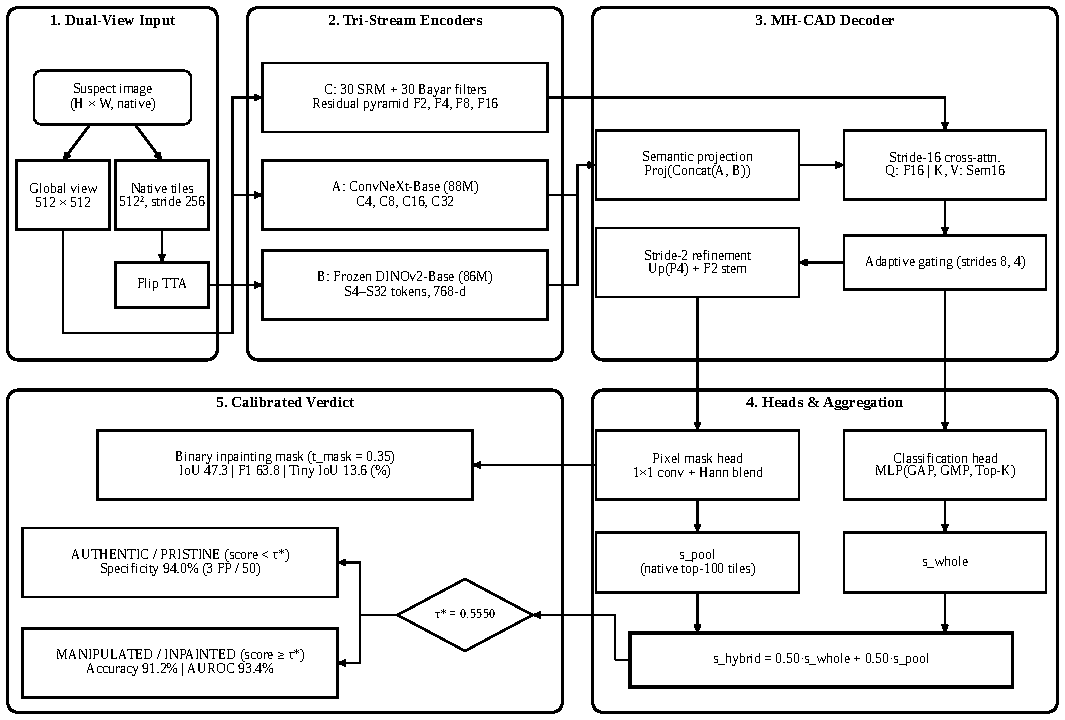
\includegraphics[width=0.85\textwidth]{figures/pipeline_flowchart_halfpage.pdf}
\caption{Overall architecture and operational dataflow of the proposed FRAME framework. (1) Dual-View Input Stage: A single suspect photograph is partitioned into a resized global view for macroscopic scene reasoning and $1:1$ native-resolution sliding tiles with horizontal-flip test-time augmentation (TTA). (2) Tri-Stream Feature Encoders: Parallel representation extraction through ConvNeXt-Base (dense hierarchical semantics), frozen DINOv2-Base (self-supervised foundation tokens), and a 60-channel noise residual pyramid (30 fixed SRM + 30 learnable Bayar constrained convolutions). (3) Multi-Head Cross-Attention Decoder (MH-CAD): Forensic residual queries cross-attend to dense semantic keys and values, guided by adaptive spatial gating and Stride-2 high-pass refinement. (4) Dual Heads \& Decision Aggregation: Reconstructs full continuous heatmap $\hat{M}$ via 2D Hann window blending and computes calibrated hybrid detection score $s_{\mathrm{hybrid}}$. (5) Calibrated Deployment Verdict: Binary localization mask at threshold $t_{\mathrm{mask}}=0.35$ and global authenticity decision at threshold $\tau^*=0.5550$.}
\label{fig:framework_flowchart}
\end{figure*}

\subsection{Problem Formulation and Dual-View Partitioning}
Let $I \in \mathbb{R}^{H \times W \times 3}$ denote an observed suspect photograph with spatial dimensions $H \times W$. The formation of a localized inpainting manipulation is modeled by the forward photometric process:
\begin{equation}
    I(x) = \big(1 - M(x)\big) \cdot J(x) + M(x) \cdot \mathcal{G}_\theta\big(J(x), p\big) + \eta(x), \quad x = (u, v) \in \Omega
    \label{eq:forward_model}
\end{equation}
where $\Omega = \{1, \dots, H\} \times \{1, \dots, W\}$ denotes the discrete pixel lattice, $J(x) \in [0, 1]^3$ represents the true, uncorrupted scene radiance captured by the camera sensor, $M(x) \in \{0, 1\}$ is the binary edit support mask indicating manipulated pixels, $\mathcal{G}_\theta$ denotes a generative diffusion or flow-matching inpainting model parameterized by weights $\theta$ and conditioned on natural language prompt $p$, and $\eta(x)$ represents camera sensor noise, color filter array (CFA) demosaicing, and quantization noise. 

The objective of FRAME is to jointly predict:
\begin{enumerate}
    \item A continuous spatial manipulation probability map $\hat{M}(x) \in [0, 1]$ estimating the posterior probability $\mathbb{P}(M(x) = 1 \mid I)$;
    \item A calibrated global authenticity score $s(I) \in [0, 1]$ estimating $\mathbb{P}(y = 1 \mid I)$, where $y = 1$ denotes a manipulated image and $y = 0$ denotes an authentic photograph.
\end{enumerate}

\paragraph{Dual-View Decomposition.} Because generative inpainting introduces subtle sub-pixel boundary seams that are obliterated by whole-image downsampling, yet requires macroscopic scene context to prevent false alarms on complex textures, FRAME processes the input image through a dual-view hierarchy:
\begin{enumerate}
    \item \textbf{Global Context View ($I_{\mathrm{global}}$):} The input image is bilinearly resized to a fixed canvas $I_{\mathrm{global}} \in \mathbb{R}^{S \times S \times 3}$ ($S = 512$). This view supplies full scene context, enabling macroscopic semantic reasoning and supervising the whole-image detection head.
    \item \textbf{Native-Resolution Sliding Tile Grid ($\{P_k\}_{k=1}^K$):} To preserve uncorrupted $1:1$ pixel scale, the native image $I$ is partitioned into an overlapping grid of $K$ square tiles $P_k \in \mathbb{R}^{S \times S \times 3}$ using a spatial stride of $S_{\mathrm{stride}} = 256$ pixels. Each tile undergoes independent feature extraction and bidirectional horizontal-flip Test-Time Augmentation (TTA), ensuring that tiny high-frequency inpainting seams are inspected without interpolation distortion.
\end{enumerate}

\subsection{Tri-Stream Feature Representation}
Each view or native tile $X \in \mathbb{R}^{S \times S \times 3}$ is independently encoded by three complementary feature streams, designed to capture dense semantics, self-supervised foundation invariants, and micro-texture noise anomalies simultaneously.

\subsubsection{Semantic Stream A: Hierarchical RGB Representation}
To extract multi-scale structural and contextual representations, we employ ConvNeXt-Base~\cite{convnext} (88M parameters). ConvNeXt utilizes $7 \times 7$ depthwise separable convolutions with inverted bottleneck ratios, providing large receptive fields that model boundary continuity across spatial scales. We extract hierarchical feature maps from all four convolutional stages at strides 4, 8, 16, and 32:
\begin{equation}
    C_s = \mathcal{E}_{\mathrm{convnext}}^{(s)}(X) \in \mathbb{R}^{\frac{S}{s} \times \frac{S}{s} \times d_c^{(s)}}, \quad s \in \{4, 8, 16, 32\}
\end{equation}
where $d_c = (128, 256, 512, 1024)$ channels. To maintain numerical stability and prevent gradient divergence during small-batch fine-tuning, the earliest two stages ($C_4, C_8$) are frozen.

\subsubsection{Semantic Stream B: Self-Supervised Foundation Tokens}
While ConvNeXt captures hierarchical convolutional inductive biases, modern visual foundation models learn rich semantic priors that are invariant to low-level lighting and color shifts. We incorporate a frozen DINOv2-Base Vision Transformer (ViT-B/14, 86M parameters)~\cite{dinov2}. The patch tokens of the final transformer block provide self-supervised representations $S_{14} \in \mathbb{R}^{\frac{S}{14} \times \frac{S}{14} \times 768}$. To establish strict spatial correspondence with the convolutional stream, the DINOv2 tokens are bilinearly interpolated to matching feature dimensions:
\begin{equation}
    S_s = \mathrm{Interpolate}\big(\mathcal{E}_{\mathrm{dino}}(X), \big(\tfrac{S}{s}, \tfrac{S}{s}\big)\big) \in \mathbb{R}^{\frac{S}{s} \times \frac{S}{s} \times 768}, \quad s \in \{4, 8, 16, 32\}
\end{equation}

\subsubsection{Forensic Residual Stream C: 60-Channel Noise Pyramid}
Natural photographic sensors exhibit stationary Poisson-Gaussian shot noise and demosaicing traces. When a diffusion model inprints synthetic pixels, it reconstructs content through an iterative Langevin-type reverse drift, introducing non-stationary noise variance and high-frequency spectral phase disruptions. To isolate these micro-texture anomalies from low-frequency scene radiance, Stream C extracts a 60-channel residual pyramid using both fixed linear and learned constrained filters:
\begin{enumerate}
    \item \textbf{Fixed Spatial Rich Model (SRM) Filters (30 channels):} We apply 30 fixed high-pass linear kernels derived from steganalysis~\cite{srm}, computing horizontal, vertical, and second-order Laplacian residual derivatives across each RGB channel:
    \begin{align}
        R_{\mathrm{horiz}}(u, v) &= X(u+1, v) - X(u, v) \\
        R_{\mathrm{vert}}(u, v) &= X(u, v+1) - X(u, v) \\
        R_{\mathrm{Laplace}}(u, v) &= \nabla^2 X(u, v) = \sum_{i, j \in \{-1, 0, 1\}} K_{\mathrm{Lap}}(i, j) X(u+i, v+j)
    \end{align}
    \item \textbf{Learned Bayar Constrained Convolutions (30 channels):} To adaptively extract non-linear residual discrepancies that escape fixed linear filters, we integrate 30 learnable constrained filters~\cite{bayar}. Each Bayar kernel $w_k \in \mathbb{R}^{5 \times 5}$ is subject to an adaptive zero-sum constraint enforced during every forward pass:
    \begin{equation}
        \tilde{w}_k(i, j) = 
        \begin{cases}
            -1, & \text{if } i = 0, j = 0 \\
            \dfrac{w_k(i, j)}{\sum_{(u, v) \neq (0, 0)} |w_k(u, v)|}, & \text{if } (i, j) \neq (0, 0)
        \end{cases}
        \label{eq:bayar_constraint}
    \end{equation}
\end{enumerate}
\noindent\textbf{Theoretical Justification for Eq.~\eqref{eq:bayar_constraint}:} The constraint $\sum_{(i, j) \neq (0, 0)} \tilde{w}_k(i, j) = 1$ with $\tilde{w}_k(0, 0) = -1$ mathematically forces the filter to predict the center pixel from its immediate spatial neighborhood:
\begin{equation}
    (X * \tilde{w}_k)(u, v) = \left( \sum_{(i, j) \neq (0, 0)} \tilde{w}_k(i, j) X(u+i, v+j) \right) - X(u, v)
\end{equation}
For smooth, natural image radiance where $X(u+i, v+j) \approx X(u, v)$, the expected filter response is strictly zero: $\mathbb{E}[(X * \tilde{w}_k)] \approx 0$. Consequently, the filter completely suppresses semantic scene content, forcing the convolutional weights to overfit exclusively to high-frequency noise variance and inpainting boundary discontinuities.

The combined 60-channel residual features are processed through four residual blocks with Group Normalization and GELU activations, yielding a multi-scale forensic pyramid:
\begin{equation}
    F_s = \mathcal{E}_{\mathrm{forensic}}^{(s)}(X) \in \mathbb{R}^{\frac{S}{s} \times \frac{S}{s} \times d_f^{(s)}}, \quad s \in \{2, 4, 8, 16\}
\end{equation}
with channels $d_f = (48, 96, 144, 192)$.

\subsection{Multi-Head Cross-Attention Decoder (MH-CAD)}
A naive concatenation of forensic noise residuals with semantic features introduces severe false alarms: complex natural textures (such as animal fur or foliage) contain high residual energy that simple feed-forward layers mistake for synthetic artifacts. To resolve this ambiguity, we formulate the Multi-Head Cross-Attention Decoder (MH-CAD).

At each pyramid scale $s \in \{4, 8, 16, 32\}$, the two semantic representations are concatenated and projected to a uniform decoder dimension $D = 128$:
\begin{equation}
    Sem_s = \mathrm{GELU}\big(\mathrm{GN}\big(\mathrm{Conv}_{1 \times 1}([C_s \parallel S_s])\big)\big) \in \mathbb{R}^{\frac{S}{s} \times \frac{S}{s} \times D}
\end{equation}
where $\parallel$ denotes channel-wise concatenation.

\subsubsection{Stride-16 Forensic Cross-Attention}
At stride 16, where macroscopic context and semantic object boundaries are established, we introduce an 8-head cross-attention mechanism. Crucially, the \textbf{forensic residual tokens act as Queries ($Q$)}, while the \textbf{dense semantic tokens act as Keys ($K$) and Values ($V$)}:
\begin{equation}
    Q = W_Q F_{16}, \quad K = W_K Sem_{16}, \quad V = W_V Sem_{16}
\end{equation}
The attended feature representation $H_{16}$ is computed as:
\begin{equation}
    H_{16} = \mathrm{Softmax}\left(\frac{Q K^T}{\sqrt{d_k}}\right) V + Q
    \label{eq:cross_attn}
\end{equation}
\noindent\textbf{Theoretical Justification for Eq.~\eqref{eq:cross_attn}:} By assigning forensic residuals to the query role, anomalous noise tokens actively query the semantic feature space to determine whether a local noise inconsistency aligns with an unnatural object boundary. In genuine textured surfaces, the semantic keys and values exhibit high mutual consistency that dissipates the attention weights, naturally suppressing false alarms.

\subsubsection{Top-Down Feature Pyramid and Stride-2 Refinement}
The attended representation $H_{16}$ is fused with $Sem_{16}$ via an adaptive spatial gate $\mathcal{G}_{16} \in [0, 1]$:
\begin{align}
    \mathcal{G}_{16} &= \sigma\Big(\mathrm{Conv}_{1 \times 1}\big(\mathrm{GELU}\big(\mathrm{Conv}_{3 \times 3}([Sem_{16} \parallel H_{16}])\big)\big)\Big) \\
    P_{16} &= \mathcal{G}_{16} \odot Sem_{16} + (1 - \mathcal{G}_{16}) \odot H_{16}
\end{align}
The pyramid propagates top-down through strides 8 and 4, fusing upsampled features with forensic residual maps:
\begin{equation}
    P_s = \mathrm{Smooth}_s\Big(\mathcal{G}_s \odot Sem_s + (1 - \mathcal{G}_s) \odot F_s + \mathrm{Up}_{2\times}(P_{2s})\Big), \quad s \in \{8, 4\}
\end{equation}
Finally, to preserve crisp sub-pixel boundary silhouettes, $P_4$ is upsampled to stride 2 and refined by concatenating the highest-resolution residual stem $F_2$:
\begin{equation}
    P_2 = \mathrm{Conv}_{3 \times 3}\big([\mathrm{Up}_{2\times}(P_4) \parallel F_2]\big) \in \mathbb{R}^{\frac{S}{2} \times \frac{S}{2} \times 64}
\end{equation}
A final $1 \times 1$ convolution followed by bilinear upsampling produces the tile mask logits $\hat{Z} \in \mathbb{R}^{S \times S}$.

\subsubsection{Image-Level Detection Head}
To predict whole-image manipulation, the stride-32 feature map $P_{32}$ is pooled via Global Average Pooling (GAP) and Global Max Pooling (GMP). To ensure that local micro-edits contribute to the global decision, we append the mean of the top $K_p = 2048$ highest pixel logits from $\hat{Z}$:
\begin{equation}
    \mathbf{v}_{\mathrm{det}} = \big[\mathrm{GAP}(P_{32}) \parallel \mathrm{GMP}(P_{32}) \parallel \mathrm{TopKMean}_{K_p}(\hat{Z})\big] \in \mathbb{R}^{257}
\end{equation}
A 2-layer MLP with dropout maps $\mathbf{v}_{\mathrm{det}}$ to the image classification logit $z_{\mathrm{det}} \in \mathbb{R}$, yielding detection score $s = \sigma(z_{\mathrm{det}})$.

\subsection{Joint Dual-View Training Objective}
To eliminate the historical supervision mismatch where empty-mask crops were penalized under global positive labels, we formulate a joint multi-task training objective:
\begin{equation}
    \mathcal{L}_{\mathrm{total}} = \mathcal{L}_{\mathrm{whole}} + 0.5 \mathcal{L}_{\mathrm{crop}} + \mathcal{L}_{\mathrm{seg}} + 0.3 \big(\mathcal{L}_{\mathrm{bg,w}} + \mathcal{L}_{\mathrm{bg,c}}\big)
    \label{eq:total_loss}
\end{equation}
The individual loss terms are defined as follows:
\begin{enumerate}
    \item \textbf{Whole-Image Detection Loss ($\mathcal{L}_{\mathrm{whole}}$):} Supervised via binary cross-entropy using the true image label $y_{\mathrm{img}} \in \{0, 1\}$:
    \begin{equation}
        \mathcal{L}_{\mathrm{whole}} = \mathrm{BCE}\big(\sigma(z_{\mathrm{det}}^{\mathrm{whole}}), y_{\mathrm{img}}\big)
    \end{equation}
    \item \textbf{Crop Edit-Presence Loss ($\mathcal{L}_{\mathrm{crop}}$):} Supervised using the decoupled crop-presence label $y_{\mathrm{crop}} \in \{0, 1\}$, where $y_{\mathrm{crop}} = 1$ strictly if the crop contains at least one edited pixel ($\sum M_{\mathrm{crop}} > 0$):
    \begin{equation}
        \mathcal{L}_{\mathrm{crop}} = \mathrm{BCE}\big(\sigma(z_{\mathrm{det}}^{\mathrm{crop}}), y_{\mathrm{crop}}\big)
    \end{equation}
    \item \textbf{Balanced Segmentation Loss ($\mathcal{L}_{\mathrm{seg}}$):} Applied only to edit-containing crops ($y_{\mathrm{crop}} = 1$). To address extreme foreground-background class imbalance where edits occupy $<2\%$ of the crop area, we combine balanced binary cross-entropy with soft Dice loss:
    \begin{equation}
        \mathcal{L}_{\mathrm{seg}} = \mathcal{L}_{\mathrm{bce\_bal}} + \mathcal{L}_{\mathrm{Dice}}
    \end{equation}
    where soft Dice loss directly optimizes the harmonic intersection:
    \begin{equation}
        \mathcal{L}_{\mathrm{Dice}} = 1 - \frac{2 \sum_{i} \hat{p}_i M_i + \epsilon}{\sum_{i} \hat{p}_i + \sum_{i} M_i + \epsilon}, \quad \hat{p}_i = \sigma(\hat{Z}_i)
    \end{equation}
    \item \textbf{Clean Background Suppression Penalties ($\mathcal{L}_{\mathrm{bg,w}}, \mathcal{L}_{\mathrm{bg,c}}$):} To penalize spurious high-frequency false alarms on authentic content, we enforce an explicit $L_1$ penalty on predicted pixel probabilities across pristine images ($y_{\mathrm{img}} = 0$) and empty-mask background crops ($y_{\mathrm{crop}} = 0$):
    \begin{equation}
        \mathcal{L}_{\mathrm{bg}} = \frac{1}{|\Omega|} \sum_{x \in \Omega} \sigma\big(\hat{Z}(x)\big)
    \end{equation}
\end{enumerate}

\subsection{Inference and Score Aggregation}
The full inference procedure is formalized in Algorithm~\ref{alg:inference}. Given an unconstrained image $I$, the global resized view produces $s_{\mathrm{whole}}$. The sliding native tiles $\{P_k\}_{k=1}^K$ are processed with bidirectional horizontal-flip TTA, and overlapping predictions are merged using 2D Hann spatial blending weights $w(x)$ to eliminate boundary edge seams:
\begin{equation}
    \hat{M}(x) = \frac{\sum_{k=1}^K w(x - x_k) \cdot \hat{P}_k(x)}{\sum_{k=1}^K w(x - x_k)}, \quad x \in \Omega
    \label{eq:hann_blend}
\end{equation}
The pooled local anomaly score $s_{\mathrm{pool}}$ is computed as the mean of the top 100 highest pixel values in $\hat{M}$. The final hybrid decision score is formulated as:
\begin{equation}
    s_{\mathrm{hybrid}} = 0.50 \cdot s_{\mathrm{whole}} + 0.50 \cdot s_{\mathrm{pool}}
    \label{eq:hybrid_score}
\end{equation}
The image decision is obtained by thresholding $s_{\mathrm{hybrid}} \ge \tau^*$ at the frozen validation threshold $\tau^* = 0.5550$. The binary localization mask is obtained by thresholding $\hat{M}(x) \ge t_{\mathrm{mask}}$ at $t_{\mathrm{mask}} = 0.35$, followed by morphological hole filling.

\begin{algorithm}[t]
\caption{FRAME Dual-View Inpainting Detection and Localization}
\label{alg:inference}
\begin{algorithmic}[1]
\REQUIRE Suspect RGB image $I \in \mathbb{R}^{H \times W \times 3}$, Tile size $S=512$, Stride $S_{\mathrm{stride}}=256$, Mask threshold $t_{\mathrm{mask}}=0.35$, Decision threshold $\tau^*=0.5550$.
\ENSURE Calibrated image decision $Y \in \{0, 1\}$, Binary localization mask $\hat{B} \in \{0, 1\}^{H \times W}$, Manipulation heatmap $\hat{M}$.
\STATE // Stage 1: Global Macro-Context Evaluation
\STATE $I_{\mathrm{global}} \leftarrow \mathrm{Resize}(I, (S, S))$
\STATE $[z_{\mathrm{det}}^{\mathrm{whole}}, \_] \leftarrow \mathrm{FRAME\_Forward}(I_{\mathrm{global}})$
\STATE $s_{\mathrm{whole}} \leftarrow \sigma(z_{\mathrm{det}}^{\mathrm{whole}})$
\STATE // Stage 2: Native-Resolution Overlapping Tile Extraction
\STATE Extract tile coordinates $\{(x_k, y_k)\}_{k=1}^K$ using stride $S_{\mathrm{stride}}$
\STATE Initialize accumulator $\hat{A} \leftarrow \mathbf{0}^{H \times W}$, Weight accumulator $\hat{W} \leftarrow \mathbf{0}^{H \times W}$
\FOR{$k = 1$ to $K$}
    \STATE $P_k \leftarrow I[y_k:y_k+S, x_k:x_k+S]$
    \STATE $[\_, \hat{Z}_k] \leftarrow \mathrm{FRAME\_Forward}(P_k)$
    \STATE $[\_, \hat{Z}_k^{\mathrm{flip}}] \leftarrow \mathrm{FRAME\_Forward}(\mathrm{FlipLR}(P_k))$
    \STATE $\hat{p}_k \leftarrow 0.5 \cdot \big(\sigma(\hat{Z}_k) + \mathrm{FlipLR}(\sigma(\hat{Z}_k^{\mathrm{flip}}))\big)$
    \STATE $\hat{A}[y_k:y_k+S, x_k:x_k+S] \mathrel{+}= \hat{p}_k \odot w_{\mathrm{Hann}}$
    \STATE $\hat{W}[y_k:y_k+S, x_k:x_k+S] \mathrel{+}= w_{\mathrm{Hann}}$
\ENDFOR
\STATE // Stage 3: Spatial Reconstruction \& Score Aggregation
\STATE $\hat{M} \leftarrow \hat{A} \oslash \hat{W}$ \COMMENT{Pointwise normalization}
\STATE $s_{\mathrm{pool}} \leftarrow \mathrm{Mean}\big(\mathrm{Top100Pixels}(\hat{M})\big)$
\STATE $s_{\mathrm{hybrid}} \leftarrow 0.50 \cdot s_{\mathrm{whole}} + 0.50 \cdot s_{\mathrm{pool}}$
\STATE $Y \leftarrow \mathbb{I}(s_{\mathrm{hybrid}} \ge \tau^*)$
\STATE $\hat{B} \leftarrow \mathrm{MorphologicalFill}\big(\mathbb{I}(\hat{M} \ge t_{\mathrm{mask}})\big)$
\RETURN $Y, \hat{B}, \hat{M}$
\end{algorithmic}
\end{algorithm}
